\documentclass[runningheads]{llncs}
%
\usepackage[T1]{fontenc}
\usepackage{graphicx}
\usepackage{amsmath,amssymb}
\usepackage{booktabs}
\usepackage{multirow}
\usepackage{array}
%
\emergencystretch=3em
\begin{document}
%
\title{GIS-Based Smart Village Infrastructure Planning Using DINOv2 Segmentation, Graph-Based Connectivity Analysis, and A$^{*}$ Route Planning}
%
\titlerunning{GIS-Based Smart Village Infrastructure Planning}
%
\author{Ramakrishna Kolikipogu\and Pendyala Archana\and Palamakula Swathi}
%
\authorrunning{R. Kolikipogu et al.}
%
\institute{Department of Information Technology, Chaitanya Bharathi Institute of Technology (A), Hyderabad, India\\
\email{krkrishna.cse@gmail.com}\\
\email{pendyalaarchanareddy98@gmail.com}\\
\email{swathip\_it@cbit.ac.in}}
%
\maketitle
%
\begin{abstract}
Rural infrastructure planning matters for living standards, but field-survey approaches are slow and hard to scale. This paper presents StrongDINOv2Seg, coupling a DINOv2 vision-transformer encoder with an FPN, Atrous Spatial Pyramid Pooling (ASPP), and a residual decoder to segment LoveDA imagery into its seven semantic classes. Trained for 10 epochs on combined Rural/Urban LoveDA, the model reaches a best validation mIoU of 53.80\% and mDice of 68.91\% at epoch 4 (no test-set evaluation was performed; epoch selection used the same split). An OpenCV/NetworkX/SciPy stage then performs building detection, road skeletonization, graph construction, KD-tree connectivity, and A$^{*}$ route planning over a land-cover-weighted cost surface, generating raster-based computational connectivity proposals for isolated buildings. On a representative tile with 14 buildings, connectivity rises from 28.57\% to 100\% via 10 proposed segments. Over 100 LoveDA Rural validation-split tiles (512 buildings), planning is possible on 19 tiles whose predicted road network is non-empty; there, connectivity rises from 13.26\% to 100\% (mean path efficiency 0.921), while 26 tiles with buildings but no detected road remain at 0\%. Terrain-aware A$^{*}$ achieves lower cost-surface traversal cost than unweighted A$^{*}$ and straight-line routes on all 19 tiles (paired Wilcoxon, $p<10^{-5}$); this validates adherence to the cost model, not real-world optimality. Off-the-shelf SegFormer-B2 and DeepLabV3-R101 are benchmarked for inference latency only. Results are validation-split, pixel-space pre-feasibility proposals, not field-validated and not establishing engineering, terrain, environmental, cost, legal, or social feasibility.
\keywords{DINOv2 \and Semantic segmentation \and ASPP \and FPN \and LoveDA dataset \and Smart village \and Rural infrastructure planning \and Road extraction \and Building detection \and Connectivity analysis \and KD-tree \and A$^{*}$ path planning \and OpenCV}
\end{abstract}
%
\section{Introduction}
Characterising rural infrastructure -- roads, buildings, water, agricultural land -- matters for living standards~\cite{hinton1996}. Poor road connectivity is a recognised barrier to healthcare access~\cite{verma2020}, and infrastructural gap analysis has been used to prioritise rural investment~\cite{kapoor2021}. GIS-based imagery analysis supports this, but manual survey is slow and hard to scale; benchmarks such as SpaceNet~\cite{vanetten2018} and DeepGlobe~\cite{demir2018} have driven progress in automated extraction, motivating its combination with planning.

This paper describes StrongDINOv2Seg: a DINOv2-based segmentation model paired with a downstream pipeline -- road extraction, skeletonization, graph construction, KD-tree connectivity, and A$^{*}$ route planning -- that turns segmentation into raster-based computational connectivity proposals. It is evaluated on LoveDA segmentation quality, a representative planning tile, a connectivity-radius sensitivity analysis, and a 100-tile planning evaluation with routing baselines and a backbone latency benchmark.

\section{Related Work}
\textbf{Segmentation.} SegFormer~\cite{xie2021} and UNetFormer~\cite{wang2022unet} (on LoveDA) advanced transformer segmentation but need large labelled sets; DINOv2~\cite{oquab2023} is self-supervised but not built for dense satellite classification, addressed here via fine-tuning with an ASPP/FPN decoder. \textbf{Road/building extraction.} D-LinkNet~\cite{zhou2018} won the DeepGlobe road-extraction challenge; attention, atrous/strip, fusion, and dual-decoder extractors followed~\cite{bai2025,ma2026,zhang2024,qu2025}, with several targeting road topology~\cite{kamada2021,mattyus2017,xu2023,liu2017}. Ayala et al.~\cite{ayala2021} jointly detected buildings and roads from Sentinel imagery, mirroring our two-class task; VHR building/settlement classification~\cite{dimassi2024,kakooei2026}, a modified ViT for rural land cover~\cite{wassan2025}, and MAP-Net~\cite{zhu2021} for small buildings are also relevant. \textbf{GIS planning and routing.} OSMnx~\cite{boeing2017} popularised the NetworkX street-graph used in our connectivity stage; Verma and Dash~\cite{verma2020} modelled rural healthcare accessibility via GIS network analysis, and Kapoor et al.~\cite{kapoor2021} ranked Telangana village infrastructure gaps, both relevant to prioritising isolated buildings. Wang et al.~\cite{wang2022astar} proposed weighted, cost-aware A$^{*}$ routing, related to our traversal-cost surface. These works generally treat segmentation, extraction, or GIS accessibility in isolation.

\textbf{Problem and contributions.} A pipeline that only classifies land cover does not, by itself, tell a planner where new access roads are needed. Planning requires a rural land-cover segmenter, a discrete inventory of buildings and roads, and a rule for deciding which buildings need access and where; prior systems address these separately. This paper integrates them as an engineering decision-support demonstration whose outputs are raster-based computational connectivity proposals, not field-validated engineering plans. The main contributions are: (i) integrating a DINOv2-based segmentation model with an explicit cost-weighted A$^{*}$ route-planning stage; (ii) class-wise and aggregate segmentation metrics; (iii) an explicit A$^{*}$ traversal-cost surface; (iv) a 100-tile planning evaluation with active-road subset statistics, paired comparisons against two routing baselines, and a radius-sensitivity sweep; (v) an inference-latency benchmark against two off-the-shelf backbones; and (vi) explicit limitations. No component is individually novel; the contribution is their integration.

\section{Proposed Methodology}
\subsection{Overall System Architecture}
The pipeline has two stages: StrongDINOv2Seg classifies each pixel into one of eight indices per the official LoveDA encoding (0 = no-data, ignored; 1--7 = Background, Building, Road, Water, Barren, Forest, Agriculture); a second stage then uses classical vision and graph algorithms to detect buildings, skeletonize roads, mark existing connections, and plan segments for isolated ones (Sect.~\ref{sec:setup}).

\subsection{DINOv2 Encoder, FPN, ASPP, and Decoder}
A pretrained \texttt{facebook/dinov2-base} Vision Transformer with patch size 14 serves as the fine-tuned encoder. Inputs are resized to $560\times560$ and embedded into $40\times40$ patch tokens. Hidden states are taken from layers 3, 6, 9, and 12 (768-dimensional each):
\begin{equation}
z'_l=\mathrm{MSA}(\mathrm{LN}(z_{l-1}))+z_{l-1},\qquad z_l=\mathrm{MLP}(\mathrm{LN}(z'_l))+z'_l
\end{equation}
where MSA is multi-head self-attention, LN is layer normalisation, and MLP is the feed-forward block. Each $40\times40\times768$ feature map is projected to 256 channels ($P_l=\mathrm{Conv}_{1\times1}(f_l)$), concatenated, and fused:
\begin{equation}
F_{\mathrm{fuse}}=\mathrm{Conv}_{1\times1}\big(\mathrm{Concat}(P_3,P_6,P_9,P_{12})\big)
\end{equation}
ASPP is applied with dilation rates 6, 12, 18, a $1\times1$ branch, and a global-pooling branch, giving a 256-channel output: $\mathrm{ASPP}(x)=\mathrm{Proj}(\mathrm{Concat}(B_1,\dots,B_5))$. A residual decoder ($R(x)=F(x)+x$) restores spatial resolution through four $2\times$ upsampling stages ($256\to256\to128\to64\to32$ channels), producing a $640\times640$ map resized to $560\times560$, followed by a final $1\times1$ convolution to eight classes.

\subsection{Loss Function}
Training uses a composite loss:
\begin{equation}
L_{\mathrm{total}}=0.5\,L_{\mathrm{CE}}+0.4\,L_{\mathrm{Dice}}+0.1\,L_{\mathrm{boundary}},\qquad L_{\mathrm{Dice}}=1-\frac{2|P\cap G|+\epsilon}{|P|+|G|+\epsilon}
\end{equation}
where $L_{\mathrm{CE}}$ is pixel-wise cross-entropy and $L_{\mathrm{boundary}}$ is a Sobel-edge-weighted boundary term; both CE and Dice ignore the no-data index (0). An auxiliary deep-supervision loss weight is defined but inactive, since the decoder exposes no auxiliary heads.

\section{System Architecture: Connectivity Analysis and Route Planning}
\subsection{Building/Road Extraction and Connectivity Graph}
Buildings are detected via 8-connected component analysis of the Building mask (OpenCV \texttt{connectedComponentsWithStats}), discarding components under 20 px. Road pixels are cleaned by $3\times3$ closing then opening and skeletonized (scikit-image) to a one-pixel centreline, converted to an undirected NetworkX graph -- the OSMnx~\cite{boeing2017} street-graph representation -- with 8-connected edges weighted 1.0 (orthogonal) or $\sqrt2$ (diagonal). A building counts as connected if the road mask, dilated by radius $r$ (default 5 px), overlaps its expanded bounding box; for isolated buildings a KD-tree over skeleton pixels returns the nearest road pixel, or none if the skeleton is empty.

\subsection{Cost-Weighted A$^{*}$ Route Planning}
For every isolated building with a valid KD-tree target, A$^{*}$ search plans a route over an 8-connected grid, following the weighted-cost formulation adopted in GIS route-planning studies such as~\cite{wang2022astar}. Let $I(p)$ denote the predicted class index at pixel $p$:
\begin{equation}
\mathrm{cost}(p)=\begin{cases}
\infty & I(p)\in\{0,4\}\ \text{(no-data, water)}\\
1 & I(p)=3\ \text{(road)}\\
2 & I(p)=7\ \text{(agriculture)}\\
3 & I(p)=1\ \text{(background)}\\
4 & I(p)=5\ \text{(barren)}\\
5 & I(p)=2\ \text{(building)}\\
8 & I(p)=6\ \text{(forest)}
\end{cases}
\end{equation}
The search minimises $F(n)=g(n)+h(n)$ with $g$ the accumulated cost and $h$ the Euclidean heuristic; since all finite costs are $\ge1$, $h$ never overestimates, so a returned route is minimum-cost under this raster model, not a globally optimal real-world design. If A$^{*}$ fails, a straight Bresenham fallback is used; it ignores the cost surface and may cross infinite-cost pixels (e.g., water), so fallback routes are topological placeholders requiring manual re-routing, not traversable proposals. Lengths are reported in pixels on the $560\times560$ grid. LoveDA imagery has a native ground sampling distance of about $0.3$\,m at $1024\times1024$~\cite{wang2021loveda}, so after resizing the effective GSD is roughly $0.3\times1024/560\approx0.55$\,m/px; for example, the 202.99 px mean proposed length on the representative tile is approximately 111\,m. These conversions are approximate and unused in any reported metric. Routes remain pixel-space decision-support proposals, not field validated, and establish no engineering, terrain, environmental, cost, legal, or social feasibility.

\begin{table}[t]
\caption{Training configuration.}\label{tab:train}
\centering
\begin{tabular}{llll}
\toprule
Parameter & Value & Parameter & Value\\
\midrule
Encoder & DINOv2-base (p14) & Optimizer & AdamW\\
Resolution/classes & $560^2$ / 8 & Weight decay & $1\times10^{-4}$\\
Batch/epochs & 2 / 10 & Grad. clip/AMP & 1.0 / off\\
Enc./dec. LR & $5\times10^{-6}$ / $5\times10^{-5}$ & Loss (CE/Dice/bnd.) & .5/.4/.1\\
LR schedule & Cosine, $\eta_{\min}=10^{-7}$ & Parameters & 93.8M\\
\bottomrule
\end{tabular}
\end{table}

\subsection{Routing Baselines and Evaluation Protocol}\label{sec:baselines}
Two baselines route each isolated building to the same KD-tree target as the proposed method. \emph{Unweighted A$^{*}$} runs on the same grid with unit step cost (1 orthogonal, $\sqrt2$ diagonal) restricted to finite-cost pixels, i.e. it avoids water and no-data but ignores land-cover differences. \emph{Euclidean line} is the Bresenham line between the building centroid and the target. Every route is scored on the proposed cost surface of Eq.~(4): the traversal cost is the sum over steps of the cost of the entered pixel times step length, with an impassable pixel charged a fixed penalty of 50 per unit step so that straight lines crossing water remain comparable. The obstacle-violation rate of a route is the percentage of its pixels whose predicted class is water or no-data. Per tile, each quantity is averaged over that tile's routes, and a tile without routes contributes 0. Because the proposed planner minimises exactly this cost surface, and obstacles are defined on the same predicted mask the planner treats as impassable, these comparisons verify cost-surface adherence and obstacle avoidance under the model; they are not independent evidence of real-world route quality. Unweighted-A$^{*}$ violations were not logged.

\subsection{Evaluation Metrics}
Segmentation uses pixel accuracy (non-background), precision, recall, F1, mIoU, and mDice, macro-averaged over the seven LoveDA classes (indices 1--7). Planning uses connectivity before/after planning, proposed-connection count, total/average road length, average nearest-road distance, and path efficiency (straight-line to planned-path ratio; 1 is most direct). Paired per-tile comparisons use medians with interquartile ranges and the exact two-sided Wilcoxon signed-rank test.

\section{Dataset, Preprocessing, and Experimental Setup}\label{sec:setup}
Data come from LoveDA~\cite{wang2021loveda} (Rural + Urban combined), a benchmark alongside SpaceNet~\cite{vanetten2018} and DeepGlobe~\cite{demir2018}. Images/masks are resized from $1024\times1024$ ($\approx0.3$\,m/px) to $560\times560$ ($\approx0.55$\,m/px; nearest-neighbour for masks), scaled to $[0,1]$ without ImageNet normalisation, with random horizontal/vertical flips and $0^\circ/90^\circ/180^\circ/270^\circ$ rotations at training only. Masks follow the official LoveDA label encoding; index 0 (no-data) is excluded from loss and metrics, and the seven scored classes are Background, Building, Road, Water, Barren, Forest, and Agriculture. The Train split was used for training and the Val split for all reported segmentation metrics; epoch selection was also made on validation mIoU, so reported metrics are model-selection-biased and no held-out test set was used.

\emph{Planning tiles.} The planning evaluation uses 100 LoveDA Rural validation-split tiles (\texttt{2522.png}--\texttt{2621.png}), which were not used for training; because the validation split guided epoch selection, they are not a held-out test set. The segmentation metrics in Table~\ref{tab:seg} are computed over the full validation split, not over these 100 tiles, and per-tile segmentation accuracy was not computed, so the planning results describe pipeline behaviour under the model's predictions. The representative tile (4216) comes from the unlabelled LoveDA Test/Rural directory and contributed to neither training nor epoch selection.

The pipeline is implemented in Python (PyTorch, Hugging Face transformers, OpenCV, scikit-image, NetworkX, SciPy, and Matplotlib) with \texttt{facebook/dinov2-base} as encoder. Training used an NVIDIA RTX A4000 GPU (16 GB); planning and the latency benchmark ran on an NVIDIA Tesla T4. Table~\ref{tab:train} lists the training configuration. The model trained end-to-end for 10 epochs (encoder at reduced LR), checkpointed on validation-mIoU improvement; epoch 4 (mIoU 0.5380, mDice 0.6891) was selected. The connectivity radius was 5 px and the minimum building area 20 px throughout, except in the radius sweep, which was run on a separate tile (4208).

\begin{table}[t]
\caption{Per-class and overall (macro-averaged) segmentation metrics on the LoveDA validation split, epoch-4 model.}\label{tab:seg}
\centering
\begin{tabular}{lrrrr}
\toprule
Class & IoU (\%) & Precision (\%) & Recall (\%) & F1 (\%)\\
\midrule
Background & 54.00 & 62.09 & 80.57 & 70.13\\
Building & 66.77 & 78.77 & 81.43 & 80.08\\
Road & 56.44 & 82.46 & 64.14 & 72.15\\
Water & 71.91 & 84.65 & 82.69 & 83.66\\
Barren & 30.13 & 49.47 & 43.52 & 46.31\\
Forest & 39.86 & 61.51 & 53.11 & 57.00\\
Agriculture & 57.50 & 87.58 & 62.61 & 73.02\\
\midrule
Overall (macro avg.) & 53.80 (mIoU) & 72.36 & 66.87 & 68.91 (mDice)\\
\bottomrule
\end{tabular}
\end{table}

\begin{figure}[t]
\centering
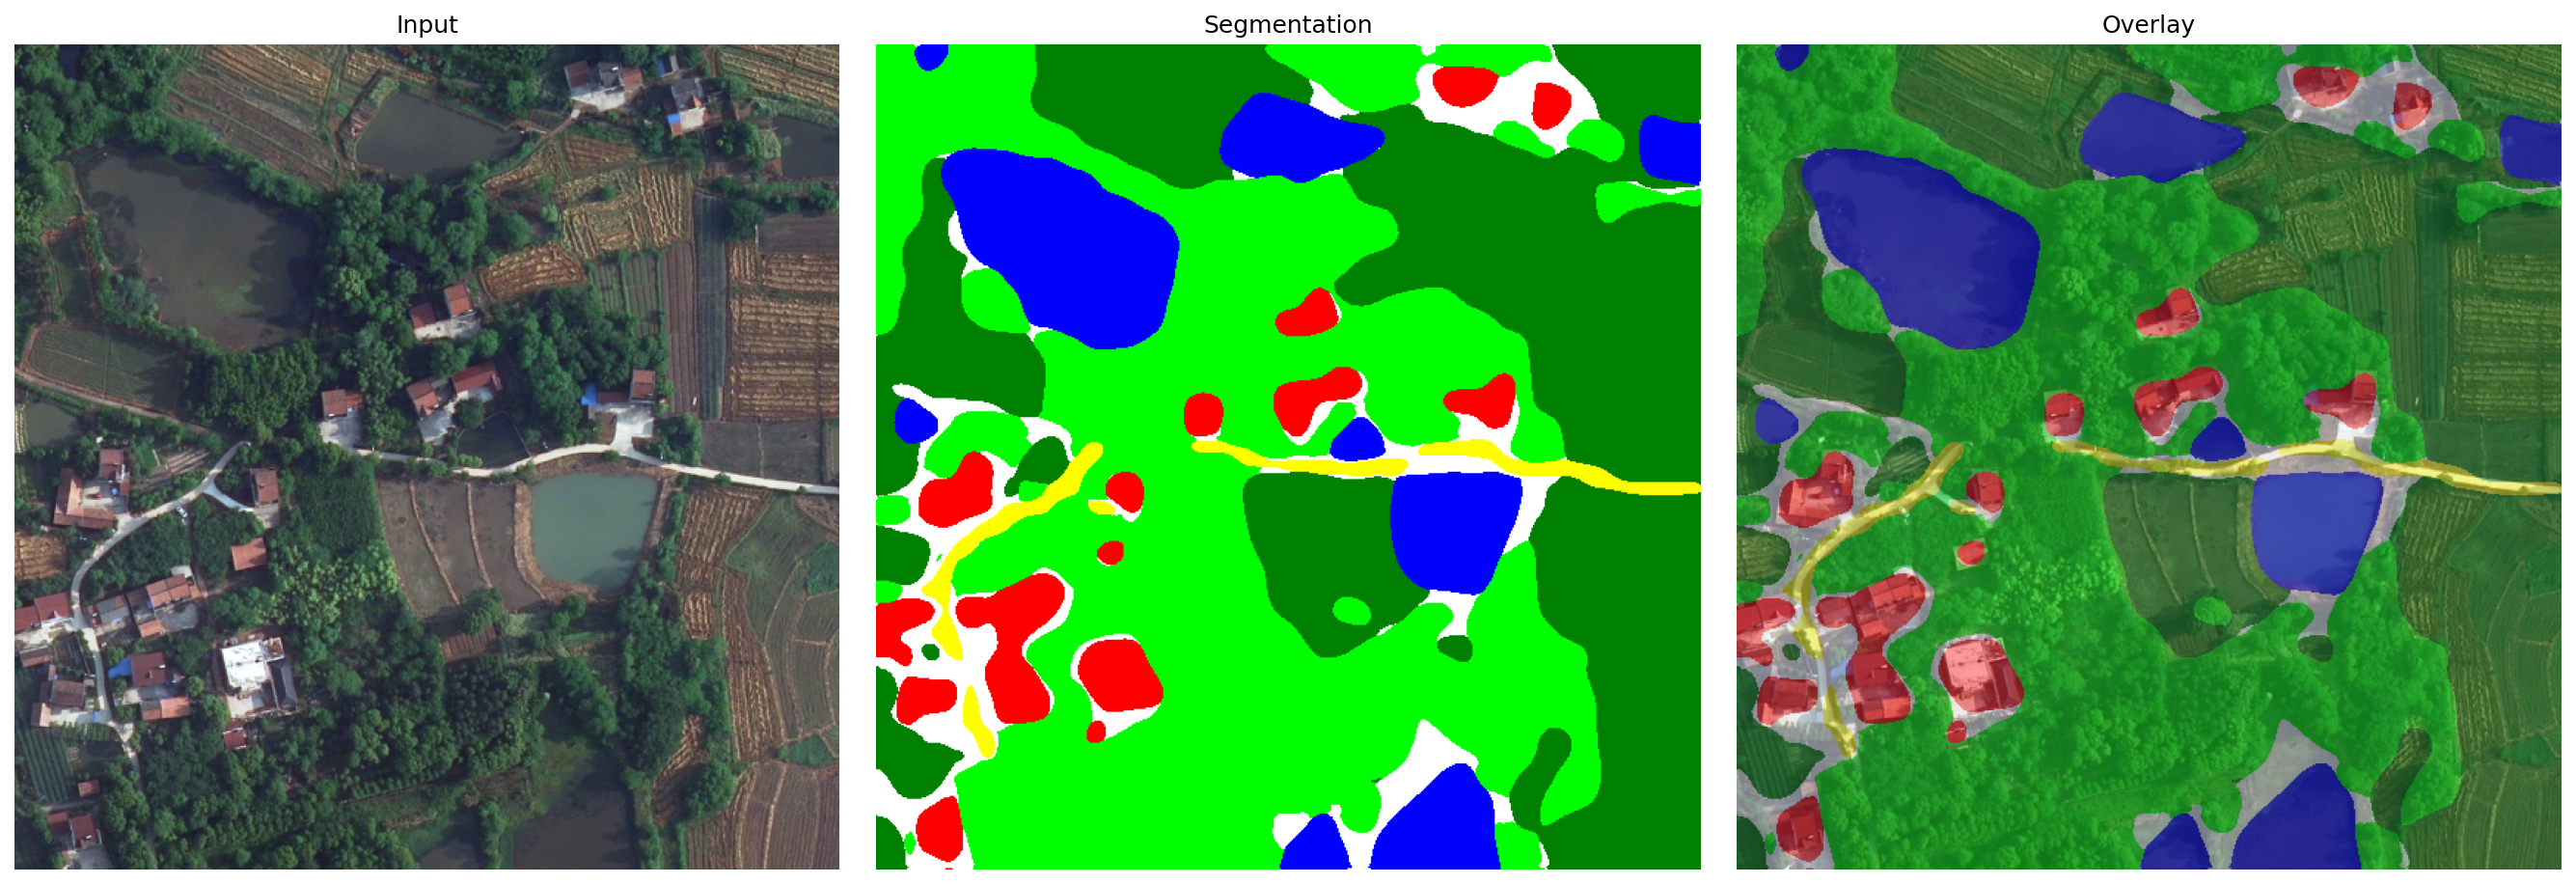
\includegraphics[width=\textwidth]{figs/fig1_segmentation.png}
\caption{Segmentation output for a sample tile. Left: input image. Centre: predicted class map. Right: prediction overlaid on the input.}\label{fig:seg}
\end{figure}

\section{Results and Discussion}
\subsection{Building Detection and Segmentation Results}
On tile 4216, 8-connected component analysis of the Building mask (20-pixel minimum area) yields 14 building instances; at $r=5$ px, 4 connect to the extracted road skeleton and 10 are isolated (Fig.~\ref{fig:plan}, left). Table~\ref{tab:seg} reports per-class and overall metrics of the epoch-4 model on the validation split: 53.80\% mIoU, 68.91\% mDice, with Building and Road IoU of 66.77\% and 56.44\% (pixel accuracy 71.34\%; Fig.~\ref{fig:seg}). Accuracy peaked at 72.19\% at epoch 2, but epoch 4 was kept since mIoU was the selection criterion. Training loss fell monotonically over 10 epochs (2.0436 to 1.0488); validation mIoU rose from 0.5208 to a peak of 0.5380 at epoch 4 before plateauing (Fig.~\ref{fig:train}).

\begin{figure}[t]
\centering
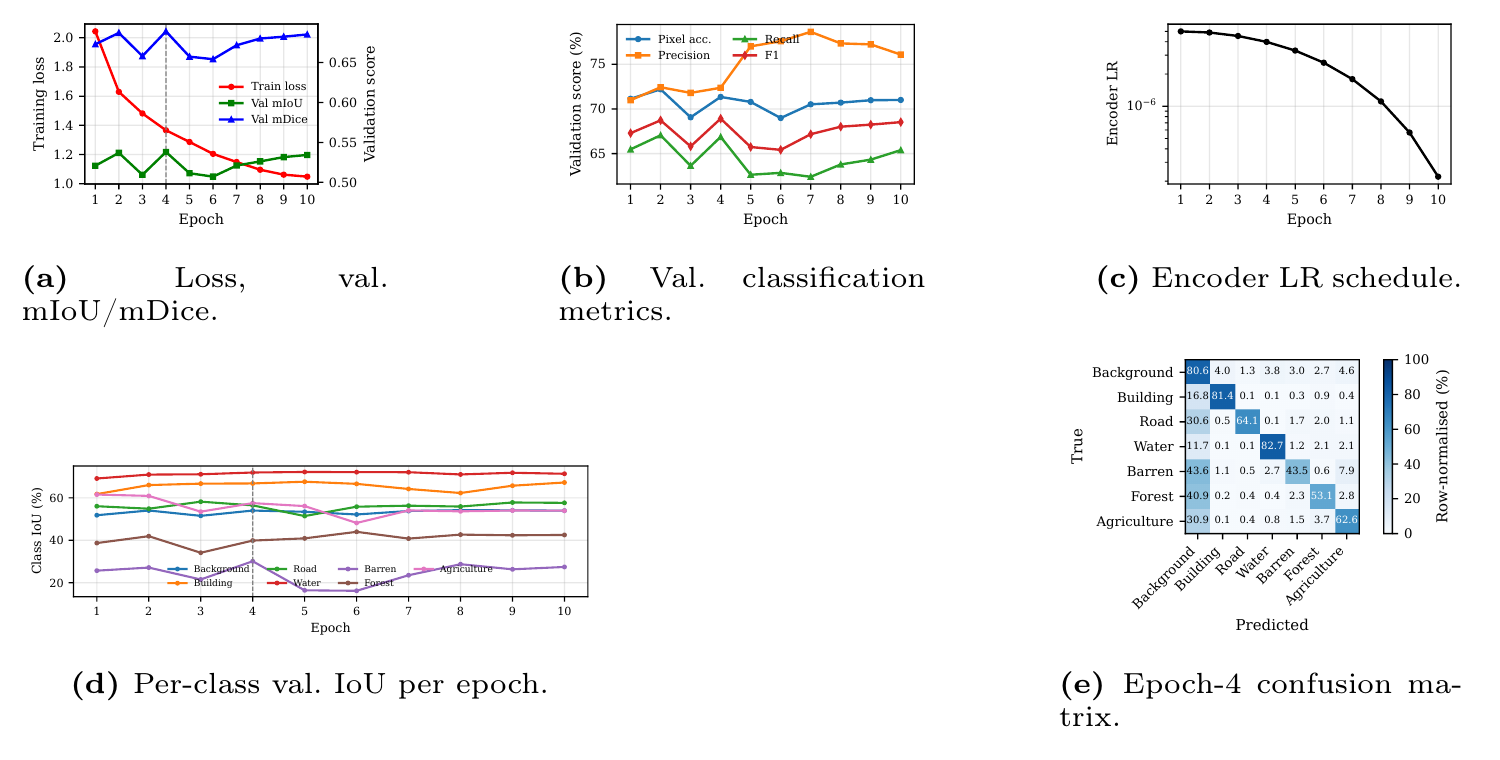
\includegraphics[width=0.92\textwidth]{figs/fig2_training.png}
\caption{Training diagnostics over ten epochs, re-plotted from the training log with official LoveDA class names: (a) loss and validation mIoU/mDice, (b) validation classification metrics, (c) encoder LR schedule, (d) per-class validation IoU per epoch, (e) epoch-4 confusion matrix. Dashed line marks epoch 4 (selected on validation mIoU); all curves are validation-split diagnostics, not held-out test results.}\label{fig:train}
\end{figure}

\subsection{Representative Tile and Radius Sensitivity}
At $r=5$ px, connectivity on the representative tile (14 buildings) rose from 4 (28.57\%) to 14 (100.00\%) via 10 connections totalling 2,029.94 px (mean 202.99 px), mean nearest-road distance 170.78 px, mean path efficiency 0.86 (Fig.~\ref{fig:plan}, right). Table~\ref{tab:radius} varies $r\in\{3,5,8,10\}$ px on a different tile (4208; 15 buildings; 46.67\% connected, 8 connections at $r=5$ px): a larger radius marks more buildings as already connected, so connections fall from 9 to 6 and length from 1,164.0 to 1,046.1 px, efficiency staying in 0.83--0.86. This sweep covers a single tile and indicates sensitivity of the connectivity rule, not a tuned optimum.

\begin{table}[t]
\caption{Connectivity-radius sensitivity on tile 4208 (15 buildings; single demonstration tile).}\label{tab:radius}
\centering
\begin{tabular}{rrrrrr}
\toprule
$r$ (px) & Before (\%) & After (\%) & Routes & Length (px) & Eff.\\
\midrule
3 & 40.00 & 100.0 & 9 & 1164.00 & 0.8605\\
5 & 46.67 & 100.0 & 8 & 1130.10 & 0.8502\\
8 & 53.33 & 100.0 & 7 & 1074.88 & 0.8529\\
10 & 60.00 & 100.0 & 6 & 1046.06 & 0.8307\\
\bottomrule
\end{tabular}
\end{table}

\begin{figure}[t]
\centering
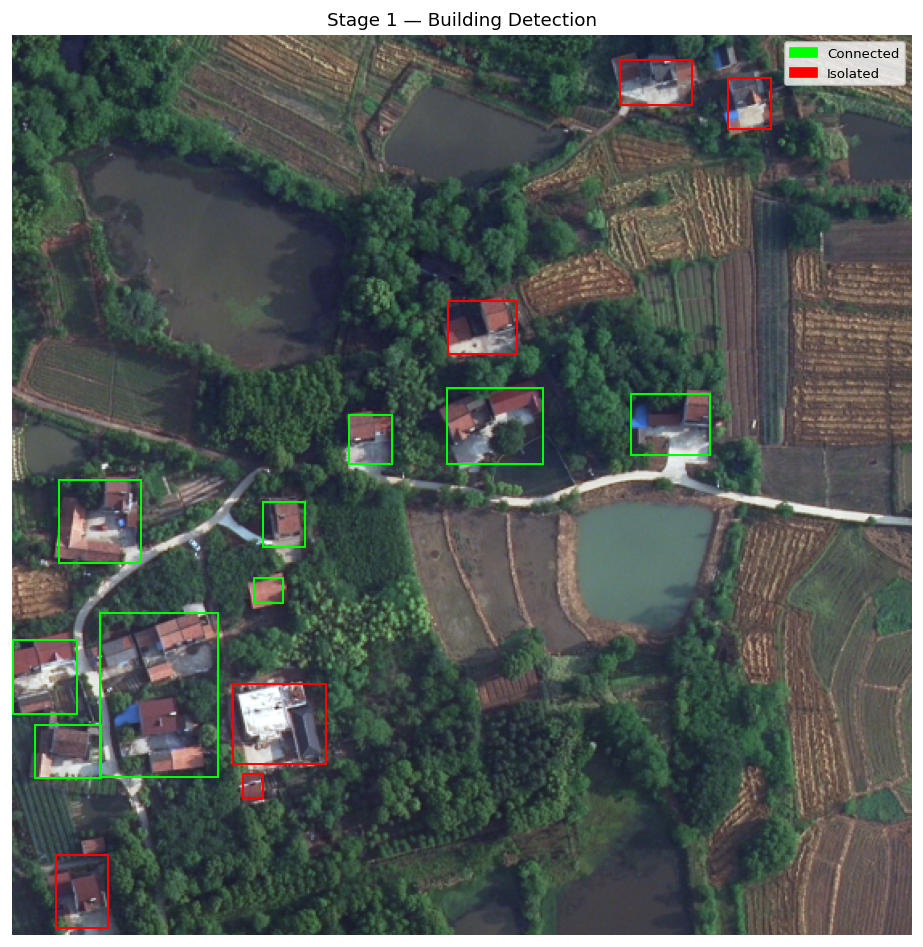
\includegraphics[width=0.48\textwidth]{figs/fig3_before.png}\hfill
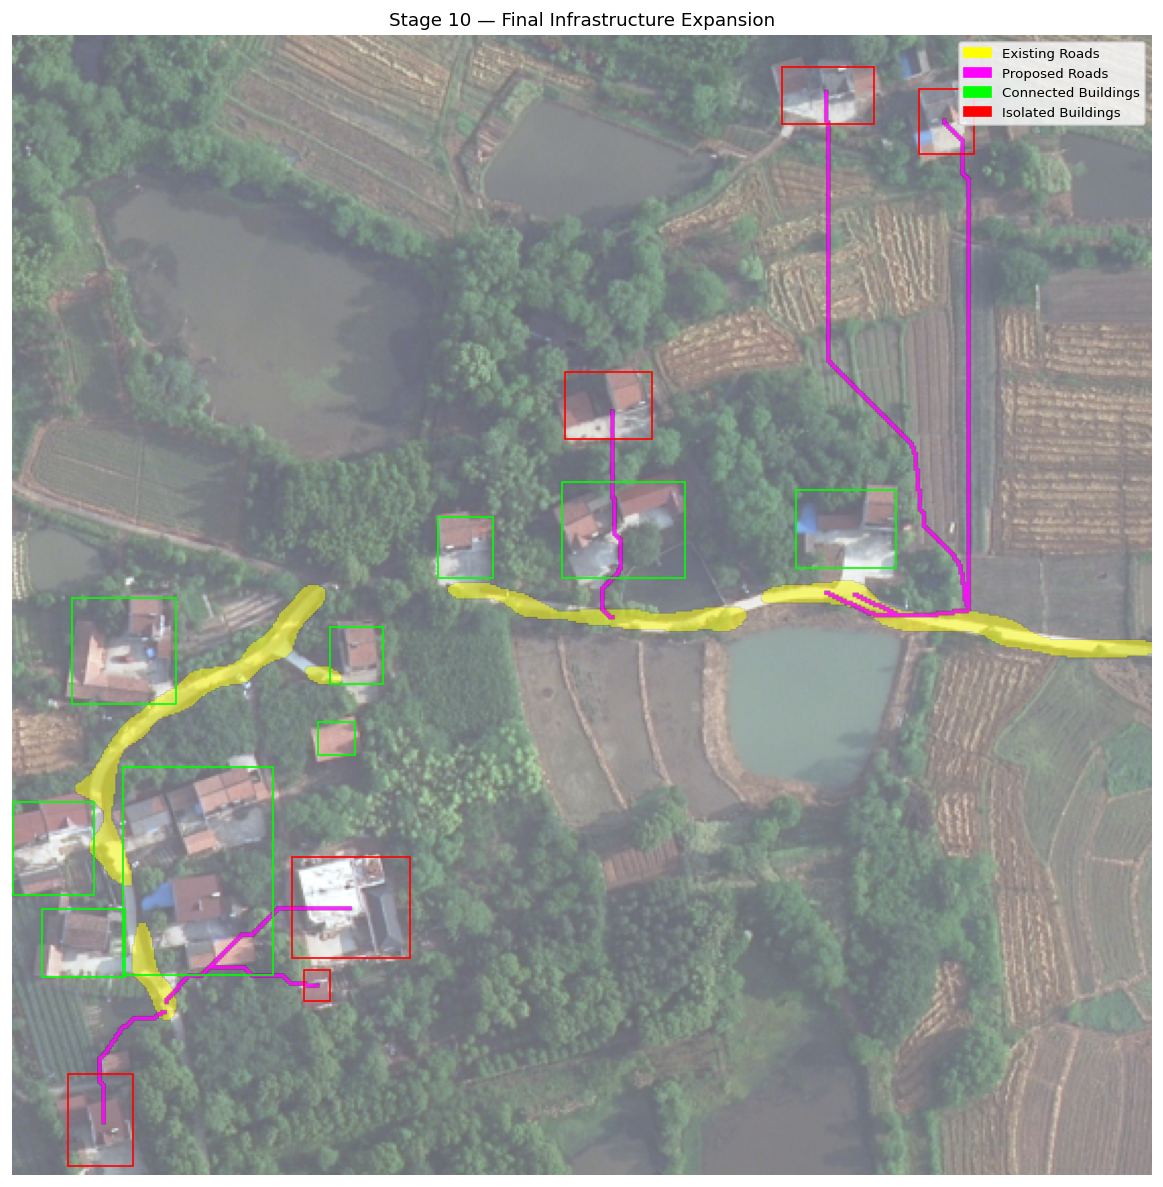
\includegraphics[width=0.48\textwidth]{figs/fig3_after.png}
\caption{Tile 4216 before (left) and after (right) planning. Green boxes: road-connected buildings (4); red: isolated (10); yellow: existing roads; magenta: A$^{*}$-planned connections.}\label{fig:plan}
\end{figure}

\subsection{Planning Evaluation on 100 Validation-Split Tiles}
Planning was run with identical settings on 100 distinct LoveDA Rural validation-split tiles (\texttt{2522.png}--\texttt{2621.png}). The tile composition is highly uneven (Table~\ref{tab:pool}). Of 100 tiles, 55 contain no detected building and 45 contain at least one (512 buildings in total). Of these 45, only 19 yield a non-empty road skeleton and hence at least one proposed route; the remaining 26 tiles (including tiles with up to 43 detected buildings) have no detected road, so the KD-tree has no target and connectivity stays at 0\%. We therefore report both all-tile statistics, which average in tiles where nothing can be planned, and statistics on the 19-tile \emph{active-road subset}, which describe planner behaviour where planning is possible. Pooled over all 512 buildings, connectivity rises from 4.88\% (25 buildings) to 36.91\% (189 buildings) via 164 proposed routes totalling 39,047 px ($\approx$21\,km at 0.55\,m/px); in the active subset it rises from 13.26\% (25 of 189) to 100\%, and all 19 active tiles reach 100\%. This 100\% is algorithmic: every isolated building with a KD-tree target receives a route, so it measures coverage by construction rather than the quality of those routes. On active tiles the mean route is 206.5 px ($\approx$113\,m) with path efficiency $0.921\pm0.021$.

\begin{table}[t]
\caption{Composition and pooled building statistics of the $N=100$ validation-split tiles (r = 5 px).}\label{tab:pool}
\centering
\begin{tabular}{lrr}
\toprule
 & All 100 tiles & Active-road subset\\
\midrule
Tiles & 100 & 19\\
Tiles with $\ge1$ detected building & 45 & 19\\
Tiles with buildings but empty road skeleton & 26 & 0\\
Buildings detected & 512 & 189\\
Connected before (pooled) & 25 (4.88\%) & 25 (13.23\%)\\
Connected after (pooled) & 189 (36.91\%) & 189 (100.00\%)\\
Isolated before & 487 & 164\\
Proposed routes / total length (px) & 164 / 39,047.4 & 164 / 39,047.4\\
\bottomrule
\end{tabular}
\end{table}

\begin{table}[t]
\caption{Per-tile planning metrics (r = 5 px): mean $\pm$ std over all 100 tiles, and over the active-road subset ($n=19$) as mean $\pm$ std and median [Q1, Q3]. All-tile path metrics include zeros for tiles with no routes.}\label{tab:n100}
\centering
\scriptsize
\setlength{\tabcolsep}{3pt}
\begin{tabular}{lrrr}
\toprule
Metric & All 100 & Active ($n=19$) & Active median [Q1, Q3]\\
\midrule
{{TAB5}}
\bottomrule
\end{tabular}
\end{table}

\subsection{Route-Planning Baselines: Cost-Surface Adherence}
Table~\ref{tab:route} compares terrain-aware A$^{*}$ with the two baselines of Sect.~\ref{sec:baselines}. On the 19 active tiles, terrain-aware A$^{*}$ has lower per-tile traversal cost than unweighted A$^{*}$ and than the Euclidean line on every tile (19/19 wins, 0 ties, 0 losses; exact two-sided Wilcoxon signed-rank $W=0$, $p=3.8\times10^{-6}$ for both comparisons). The per-tile relative cost reduction versus unweighted A$^{*}$ has median 7.6\% (IQR 3.2--11.3\%, range 0.5--19.8\%) and versus the Euclidean line median 10.5\% (IQR 7.5--15.1\%, range 0.8--75.3\%). Across all 100 tiles the mean costs are 132.9, 142.0 and 167.7, i.e.\ 6.4\% and 20.7\% lower for the proposed method, but 81 tiles have zero cost for all methods (no routes), so the paired test is only informative on the active subset. Mean standard deviations are of the order of the means because tile difficulty varies widely; the paired differences are consistent in sign.

For obstacle avoidance, the Euclidean line crosses predicted water or no-data pixels on 4 of the 19 active tiles (mean violation 0.391\% over 100 tiles, 2.06\% over active tiles), whereas the terrain-aware route does so on one tile (0.136\% over 100 tiles, 0.72\% over active tiles). On that tile (2604) the two methods report the same 13.63\%, consistent with the Bresenham fallback described in Sect.~4.2; on the other three tiles A$^{*}$ eliminated all violations. With only four affected tiles, this difference is not statistically significant (exact Wilcoxon on the 3 non-tied tiles, two-sided $p=0.25$), so we report it descriptively. Since the planner treats these pixels as impassable by construction, zero violations are expected whenever A$^{*}$ succeeds; the figures confirm the implementation honours the obstacle model rather than demonstrating performance on ground-truth water.

\begin{table}[t]
\caption{Route-planning comparison (traversal cost on the proposed cost surface; lower is better). Active subset: 19 tiles with proposed routes (mean $\pm$ std; median [Q1, Q3]); all-tile columns average over 100 tiles including zeros. Violation: \% of route pixels on predicted water/no-data.}\label{tab:route}
\centering
\scriptsize
\setlength{\tabcolsep}{2pt}
\begin{tabular}{lrrrr}
\toprule
 & \multicolumn{2}{c}{Cost, active ($n=19$)} & Cost, all 100 & Violation (\%), all 100\\
Method & mean $\pm$ std & median [Q1, Q3] & mean $\pm$ std & mean $\pm$ std\\
\midrule
{{TAB6}}
\bottomrule
\multicolumn{5}{l}{$^{\ddagger}$ Restricted to finite-cost pixels; violation rate not logged.}
\end{tabular}
\end{table}

\subsection{Backbone Inference-Latency Comparison}
To place the segmentation stage's runtime in context, we timed two publicly available segmentation backbones on the same 100 tiles at $560\times560$, batch size 1, on a Tesla T4 GPU (Table~\ref{tab:lat}). Timing covers the forward pass, the arg-max, and the transfer of the label map to the CPU, with CUDA synchronisation; no separate warm-up pass was used. The two baselines are used \emph{as released}: SegFormer-B2 fine-tuned on ADE20K and torchvision DeepLabV3-R101 with its default pretrained weights. Neither was fine-tuned on LoveDA, so they do not predict the LoveDA label set, and we make \textbf{no accuracy or segmentation-quality comparison}; the table supports only a statement about inference cost. StrongDINOv2Seg ($148.16$\,ms) is about 1.9$\times$ slower than SegFormer-B2 ($77.90$\,ms) and 27.5\% faster than DeepLabV3-R101 ($204.25$\,ms). Whether StrongDINOv2Seg's accuracy exceeds that of LoveDA-trained versions of these architectures remains untested (Sect.~\ref{sec:limits}).

\begin{table}[t]
\caption{Inference latency on 100 tiles ($560\times560$, batch 1, Tesla T4), mean $\pm$ std. Off-the-shelf baselines were not fine-tuned on LoveDA; no accuracy comparison is implied.}\label{tab:lat}
\centering
\begin{tabular}{llr}
\toprule
Model & Weights & Latency (ms)\\
\midrule
StrongDINOv2Seg (ours) & LoveDA fine-tuned (this work) & $148.16\pm33.12$\\
SegFormer-B2 & ADE20K-finetuned (HF \texttt{segformer-b2}) & $77.90\pm25.09$\\
DeepLabV3-R101 & torchvision default (COCO/VOC) & $204.25\pm57.61$\\
\bottomrule
\end{tabular}
\end{table}

\subsection{Discussion}
Water scores highest on IoU/F1 (71.91\%/83.66\%), followed by Building (66.77\%/80.08\%), in line with lightweight segmenters such as UNetFormer~\cite{wang2022unet} (benchmarks differ, so no direct comparison). Background recall (80.57\%) exceeds precision (62.09\%, over-prediction); Agriculture shows the opposite (87.58\%/62.61\%, conservative); Barren and Forest remain weakest (30.13\%/39.86\% IoU); Road's 56.44\% IoU with 64.14\% recall makes broken or missed road masks a realistic planner failure mode, and the 100-tile run shows it directly: 26 of 45 tiles with buildings produced no usable road skeleton. Missed buildings and broken roads propagate into the component analysis, skeleton graph, and A$^{*}$ planning, so the 100\% post-planning connectivity on active tiles is algorithmic, pixel-space connectivity, not field-validated infrastructure -- matching GIS accessibility studies~\cite{verma2020,kapoor2021} where network quality and prioritisation, not raw counts, determine real gains. With an empty skeleton the KD-tree has no target, so proposed-road count, length, efficiency, and nearest-road distance become the more informative outputs.

\section{Limitations and Future Work}\label{sec:limits}
\textbf{Evaluation split.} All segmentation numbers come from the LoveDA validation split, which also guided epoch selection, so no held-out test set was used and results carry model-selection bias. The 100 planning tiles are validation-split tiles that were not used for training, not a held-out test set; per-tile segmentation accuracy on them was not computed. \textbf{Baselines.} SegFormer-B2 and DeepLabV3-R101 were evaluated for latency only, using weights not fine-tuned on LoveDA; no claim of superior segmentation accuracy is made, and a like-for-like comparison would require fine-tuning them on LoveDA under the same protocol and reporting mIoU and Road IoU. Isolating the FPN, ASPP, and decoder contributions is likewise left for future work. \textbf{Routing comparison.} The routing comparison is scored on the same predicted-class cost surface that terrain-aware A$^{*}$ minimises, and obstacle violations are measured on the same predicted mask; it therefore validates cost-surface adherence and obstacle avoidance under the model, not real-world route quality. Evaluation against ground-truth masks is future work. \textbf{Planning scope and failure modes.} 100\% connectivity holds only on the 19 tiles with a non-empty predicted road network; it fails outright on 26 tiles where no road is detected, and the Bresenham fallback can cross impassable terrain. \textbf{Field validation and terrain data.} No physical on-ground survey was performed: proposed routes were not checked against GPS-measured ground truth, cadastral and land-ownership records, existing paths, or community input. No digital elevation model (DEM) was used, so slope, drainage, earthworks, and flood exposure do not enter the cost surface; water is the only terrain obstacle. Costs are heuristic class weights, not calibrated construction costs, and distances remain in pixels (with an approximate 0.55\,m/px conversion) rather than georeferenced units. The framework should therefore be read as an automated, remote-sensing pre-feasibility screening tool that can shortlist candidate connections for expert and field verification, not as an engineering design tool. \textbf{Generalisation.} 100 tiles from a single dataset split is a larger but still limited sample; Rural/Urban LoveDA domains were trained jointly without separate evaluation. Future work includes DEM-based slope costs, georeferenced planning, field and cadastral validation, ground-truth-based route evaluation, and GIS prioritisation frameworks~\cite{verma2020,kapoor2021}.

\section{Conclusion}
StrongDINOv2Seg integrates DINOv2-based segmentation, graph-based connectivity analysis, and cost-weighted A$^{*}$ planning for rural infrastructure decision support, reaching a best validation mIoU of 53.80\% and mDice of 68.91\% on Rural/Urban LoveDA. Connectivity rose from 28.57\% to 100\% on the representative tile (10 connections, efficiency 0.86). Over 100 validation-split tiles, planning was possible on 19 tiles with a detected road network, where connectivity rose from 13.26\% to 100\% (efficiency $0.921\pm0.021$) and terrain-aware A$^{*}$ was cheaper than both baselines on every tile under the cost model; on 26 further tiles with buildings no road was detected and nothing could be planned. Off-the-shelf backbones were compared for latency only. The contribution is the integrated pipeline, not any single component, and outputs are raster-based connectivity proposals suitable for pre-feasibility screening, not field-validated or construction-ready plans; LoveDA-trained baselines, ground-truth route evaluation, DEM-aware costs, and field validation are future work.

\begin{credits}
\subsubsection{\discintname}
The authors declare that they have no known competing financial interests or personal relationships that could have appeared to influence the work reported in this paper.
\end{credits}

\begin{thebibliography}{25}
\bibitem{ayala2021} Ayala, C., Sesma, R., Aranda, C., Galar, M.: A deep learning approach to an enhanced building footprint and road detection in high-resolution satellite imagery. Remote Sensing 13(16), 3135 (2021). \doi{10.3390/rs13163135}
\bibitem{bai2025} Bai, H., Ren, C., Huang, Z., Gu, Y.: A dynamic attention mechanism for road extraction from high-resolution remote sensing imagery using feature fusion. Scientific Reports 15(1), 17556 (2025). \doi{10.1038/s41598-025-02267-6}
\bibitem{boeing2017} Boeing, G.: OSMnx: New methods for acquiring, constructing, analyzing, and visualizing complex street networks. Comput. Environ. Urban Syst. 65, 126--139 (2017). \doi{10.1016/j.compenvurbsys.2017.05.004}
\bibitem{demir2018} Demir, I., Koperski, K., Lindenbaum, D., Pang, G., Huang, J., Basu, S., Hughes, F., Tuia, D., Raskar, R.: DeepGlobe 2018: A challenge to parse the earth through satellite images. In: 2018 IEEE/CVF Conference on Computer Vision and Pattern Recognition Workshops (CVPRW), pp. 172--17209. IEEE (2018). \doi{10.1109/CVPRW.2018.00031}
\bibitem{dimassi2024} Dimassi, M., Samhat, A.E., Zaraket, M., Haidar, J., Shukor, M., Ghandour, A.J.: Buildings' classification using very high-resolution satellite imagery. In: Proc. 5th Int. Electron. Conf. Remote Sens. (ECRS 2023). MDPI (2024). \doi{10.3390/ECRS2023-17969}
\bibitem{hinton1996} Hinton, J.C.: GIS and remote sensing integration for environmental applications. Int. J. Geogr. Inf. Syst. 10(7), 877--890 (1996)
\bibitem{kakooei2026} Kakooei, M., Bailie, J., Pettersson, M.B., S\"oderberg, A., Becevic, A., Daoud, A.: A high-resolution urban and rural settlement map of Africa using deep learning and satellite imagery. Scientific Reports 16(1), 637 (2026)
\bibitem{kamada2021} Kamada, S., Ichimura, T.: Automatic extraction of road networks from satellite images by using adaptive structural deep belief networks. In: Joint 10th ICIEV \& 5th icIVPR, pp. 1--7 (2021)
\bibitem{kapoor2021} Kapoor, N., Ahmad, N., Nayak, S., Singh, S., Ilavarasan, P., Ramamoorthy, P.: Identifying infrastructural gap areas for smart and sustainable tribal village development: a data science approach from India. Int. J. Inf. Manag. Data Insights 1(2), 100041 (2021). \doi{10.1016/j.jjimei.2021.100041}
\bibitem{liu2017} Liu, J., Qin, Q., Li, J., Li, Y.: Rural road extraction from high-resolution remote sensing images based on geometric feature inference. ISPRS Int. J. Geo-Inf. 6(10), 314 (2017)
\bibitem{ma2026} Ma, Y., Yu, J., Hao, Y., Chen, Y., Wang, Y., Wu, Q., et al.: Road extraction with weak features and complex backgrounds based on AtrousStripUNet. Sensors 26(4), 1134 (2026)
\bibitem{mattyus2017} Mattyus, G., Luo, W., Urtasun, R.: DeepRoadMapper: Extracting road topology from aerial images. In: Proc. IEEE Int. Conf. on Computer Vision, pp. 3438--3446 (2017)
\bibitem{oquab2023} Oquab, M., Darcet, T., Moutakanni, T., Vo, H., Szafraniec, M., Khalidov, V., et al.: DINOv2: Learning robust visual features without supervision. arXiv preprint arXiv:2304.07193 (2023)
\bibitem{qu2025} Qu, S., Liu, G., Zhang, X., Liu, Y.: Heterogeneous dual-decoder network for road extraction in remote sensing images. Scientific Reports 15(1), 31619 (2025)
\bibitem{vanetten2018} Van Etten, A., Lindenbaum, D., Bacastow, T.M.: SpaceNet: A remote sensing dataset and challenge series. arXiv preprint arXiv:1807.01232 (2018)
\bibitem{verma2020} Verma, V.R., Dash, U.: Geographical accessibility and spatial coverage modelling of public health care network in rural and remote India. PLOS ONE 15(10), e0239326 (2020). \doi{10.1371/journal.pone.0239326}
\bibitem{wang2021loveda} Wang, J., Zheng, Z., Ma, A., Lu, X., Zhong, Y.: LoveDA: A remote sensing land-cover dataset for domain adaptive semantic segmentation. arXiv preprint arXiv:2110.08733 (2021)
\bibitem{wang2022unet} Wang, L., Li, R., Zhang, C., Fang, S., Duan, C., Meng, X., Atkinson, P.M.: UNetFormer: A UNet-like transformer for efficient semantic segmentation of remote sensing urban scene imagery. ISPRS J. Photogramm. Remote Sens. 190, 196--214 (2022). \doi{10.1016/j.isprsjprs.2022.06.008}
\bibitem{wang2022astar} Wang, X., Zhang, H., Liu, S., Wang, J., Wang, Y., Shangguan, D.: Path planning of scenic spots based on improved A* algorithm. Scientific Reports 12, 1320 (2022). \doi{10.1038/s41598-022-05386-6}
\bibitem{wassan2025} Wassan, S., Bilal, A., Alzahrani, A., Almohammadi, K., Alrashidi, M., Mousavirad, S.J.: A modified vision transformer framework for image-based land cover segmentation in rural architectural design and planning. Scientific Reports 15(1), 32658 (2025). \doi{10.1038/s41598-025-19234-w}
\bibitem{xie2021} Xie, E., Wang, W., Yu, Z., Anandkumar, A., Alvarez, J.M., Luo, P.: SegFormer: Simple and efficient design for semantic segmentation with transformers. Adv. Neural Inf. Process. Syst. 34, 12077--12090 (2021)
\bibitem{xu2023} Xu, Z., Liu, Y., Sun, Y., Liu, M., Wang, L.: RNGDet++: Road network graph detection by transformer with instance segmentation and multi-scale features enhancement. IEEE Robot. Autom. Lett. 8(5), 2991--2998 (2023)
\bibitem{zhang2024} Zhang, Y., Zhang, L., Wang, Y., Xu, W.: AGF-Net: Adaptive global feature fusion network for road extraction from remote-sensing images. Complex Intell. Syst. 10(3), 4311--4328 (2024)
\bibitem{zhou2018} Zhou, L., Zhang, C., Wu, M.: D-LinkNet: LinkNet with pretrained encoder and dilated convolution for high resolution satellite imagery road extraction. In: 2018 IEEE/CVF Conference on Computer Vision and Pattern Recognition Workshops (CVPRW), pp. 182--186. IEEE (2018). \doi{10.1109/CVPRW.2018.00034}
\bibitem{zhu2021} Zhu, Q., Liao, C., Hu, H., Mei, X., Li, H.: MAP-Net: Multiple attending path neural network for building footprint extraction from remote sensed imagery. IEEE Trans. Geosci. Remote Sens. 59(7), 6169--6181 (2021). \doi{10.1109/TGRS.2020.3026051}
\end{thebibliography}
\end{document}
